%!TEX root = paper.tex
\section{System Architecture}

An important insight for Seattle as a platform is how the classical
dichotomy of service platform operators and users gives way to multi-faceted
trust relationships between a large number of mutually-unrelated
stakeholders.
In Seattle, the actual edge-based software installs, core infrastructure
services, clearinghouse operations, platform software builds, and remote
application deployments might be carried out and managed by different
groups of people, potentially untrusted (or even unknown) between groups
and among members of the same group.
% Then why/how do people trust each other in such a system?

This gives rise to a set of components~\cite{Cappos2009},
any of which useful
by itself, that can be freely combined to implement various
deployment models, from pure peer-to-peer operation up to a
provisioned deployment by a dedicated operator. Furthermore,
new components may be introduced freely to replace or augment
existing ones, as long as the component interfaces are adhered to.
We briefly introduce the default components below.
As detailed in Section~\ref{sec-deployment}, we have actively used
and developed these components over the last years as a part of
Seattle's public, live deployment.

\begin{figure}
  \centering
  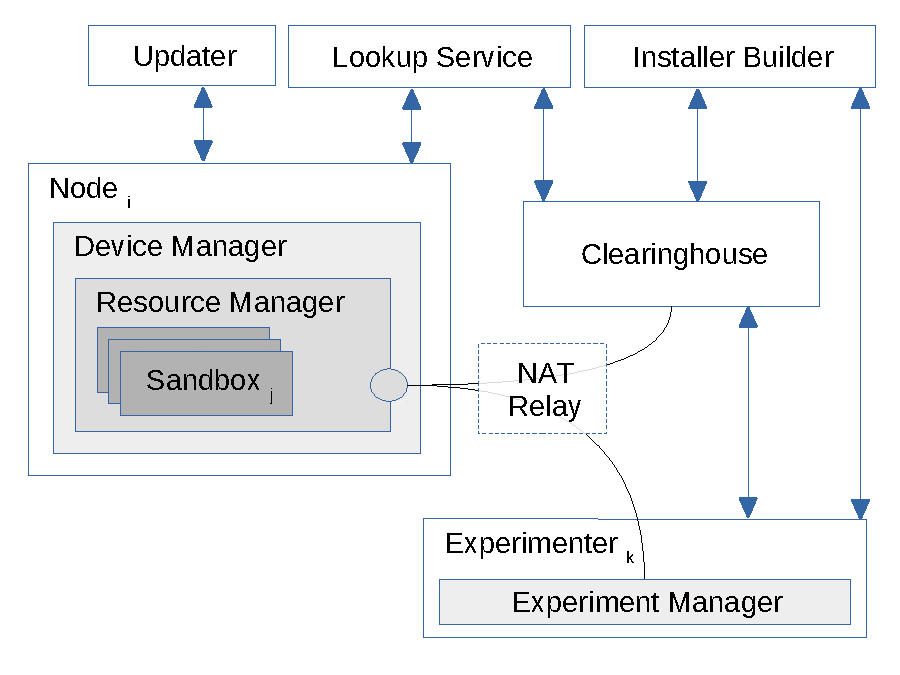
\includegraphics[width=\columnwidth]{figures/components.pdf}
  \caption{Components and interconnections of Seattle's architecture.}
  \label{fig:arch}
\end{figure}


\subsection{Components}

Figure~\ref{fig:arch} overviews Seattle's components and their
interconnections.
%The components fall into three categories: device software,
%infrastructure, and control.

We first introduce the components running on all devices that
run Seattle.
The core element of computation is a restricted,
performance- and security-isolated Python-based
\textit{Sandbox}~\cite{RepySandbox,li2015fence}.
The sandbox \gls{API} provides
networking, file, threading, etc. functions to
the code it executes. Note that
following Seattle's research and educational background, we
call code that is executed in sandboxes an ``experiment'',
regardless of its actual nature.

The \textit{Resource Manager} combines the functionality of
a hypervisor with a remote-control server.
It isolates % chroots, effectively!
sandboxes that run in
parallel, and interfaces with them on behalf of authorized remote
parties to start or stop them, upload and download data, reset
sandboxes, or transfer ownership. The sandboxes on one
device might all have different authorized users if so desired,
so that one Seattle node can serve multiple experimenters.
Due to the heterogeneity encountered in today's networks,
the Resource Manager also includes techniques to traverse
\gls{NAT} gateways and firewalls as often found in end-user
gateway routers.

The \textit{Device Manager} % (installer with \texttt{--percentage}, start/stop scripts, uninstaller, softwareupdater): device owner retains control!
is the device owner's interface to enable or disable a Seattle
install, and choose the amount of resources that it may consume on the respective
device.

The \textit{Software Updater} keeps all components of the
device software up to date. This concludes the overview of
device-side Seattle components.
%Other components are run either by experimenters, or
%infra-ops, or how should we say this so that it's exact?
\\

To control the fundamental functions of sandboxes (such as
starting to execute code, or downloading collected data),
an \textit{Experiment Manager} % (seash)
is used. The experiment manager contacts sandboxes through the
resource manager interface programmatically, and provides a
human-usable interface to the experimenter. The experimenter
authenticates against sandboxes by using cryptographic keys.

Every experimenter runs an experiment manager, and possesses
their own set of cryptographic keys. This enables interesting
deployment options (and thus applications):
Two experimenters could choose to mutually authenticate the
other on the sandboxes they control, or swap resources, and
so on; making more sandboxes available to an experiment than
a single experimenter could ever reach.
\\

Seattle's device software and an initial set of cryptographic
keys controlling the sandboxes are shipped in the form of a bundled
installer for the specific platform \gls{OS}.
The \textit{Installer Builder} component is responsible for
packaging and hosting the code and public keys.
The installer builder allows experimenters to create their own
custom installers, where they get to choose the public key or keys
that are included in the installer package. Every custom installer
can be referenced through its specific, static \gls{URL}.
Thus, by selecting and installing a specific packaged installer,
device owners can choose which experimenters to grant
access to sandboxes on their devices initially.
\\

%This sums up all of the Seattle components required for a
%self-hosted, infrastructure-less deployment already.

The default Seattle architecture also includes a
\textit{Lookup Service}. This is a generic network-accessible
key/value store that the Resource Manager and Experiment Manager
can use to announce and retrieve information about sandboxes.
For instance, a Resource Manager announces its contact information
(such as its own or a \gls{NAT} forwarder's \gls{IP} address and port number) under
the public keys of all currently authorized experimenters.
The experiment manager retrieves the contact information by looking up
the experimenter's public key at the lookup service, and then
proceeds to contact every resource manager that hosts sandboxes
that the experimenter can control.

We run \textit{\gls{NAT} Relays} on some Seattle nodes that are
accessible from the public Internet. Using these relays, firewalled
or \gls{NAT}ted nodes have a common, public meeting point to
direct Experiment Managers to.

Lastly, Seattle provides a \textit{Clearinghouse} which is a
centralized sandbox-sharing site. As motivated earlier,
sandboxes can be swapped; a clearinghouse can act as a trusted
intermediary on behalf of all registered experimenters, and creates
a large pool of sandboxes without requiring all experimenters to
set up mutual trust relationships amongst each others.
The Clearinghouse uses the same Resource Manager interfaces as the
Experiment Manager does, and provides a human-usable interface to
experimenters to request and release sandboxes.
The Clearinghouse implements internal policies
that govern the exact rules for swapping sandboxes between
registered experimenters.

This concludes the overview of Seattle components. Our live deployment
of Seattle includes implementations of all components, including a
Clearinghouse that offers free access to an initial set of sandboxes
for all registered experimenters.




\subsection{Operational Flexibility}\label{sec-op-flex}

The preceding section implicitly introduced different roles relevant
in the Seattle architecture:
\textit{device owners} control whether and how they participate
in Seattle, so as to provide sandboxes to the platform;
\textit{experimenters} use these sandboxes to run their code
on remote devices;
lastly, there are \textit{operators} for various components
of the infrastructure.
These roles match what most existing \gls{fc} architectures
foresee.
However, the limited and clearly-defined boundaries of Seattle
components result in few requirements on mutual trust or, indeed,
interaction between
the actual persons acting in these roles. This enables operational
scenarios including and exceeding the often-assumed centrally managed
and operated \gls{fc} setups.

For instance, in a local experimental deployment, the owner of all
devices might serve as the experimenter at the same time. If
the Experiment Managers and Installer Builders can be reused
from existing deployments, no additional effort is involved in
setting up the infrastructure.
A setup on exclusively-controlled, all-local devices can serve as
a testbed for research, or enables device owners to run an
``OwnCloud''-like \gls{fc} setup on their equipment.

The same approach also scales to groups of device owners and experimenters
that federate
to share resources on (parts of) their setups. No trusted
intermediary in the form of a Clearinghouse is required:
trust relationships among the researchers and the device owners
can be set up out-of-band as well.

Another realization may provide all of the components described above.
This gives a sponsored set of sandbox resources to start with,
a clearinghouse to mediate access between contributed sandboxes
and registered researches, and all of the auxiliary services
discussed. The current deployment of Seattle is an example for
this: We operate instances of all components; further instances
(particularly of sandboxes on remote nodes) are contributed and
operated by volunteers.
Section~\ref{sec-deployment} details our current deployment.

Sensibility Testbed~\cite{zhuang2014sensibility} and Social Compute
Cloud~\cite{caton2014social} provide a similar breadth in capabilities
as Seattle. However, they only operate a partial infrastructure, and
reuse much of Seattle's. Their own Clearinghouse
implementations have user interfaces and policy implementations
that differ from Seattle's. Sensibility also provides a new sandbox
type that allows privacy-preserving access to sensors on Android
smartphones and tablets. Other components, including the Experiment
Manager, are reused unchanged.

Finally, we envision that multiple central operators (as often
assumed in \gls{fc}) could set up their own instances of
all components, and then federate using Seattle's open interfaces
to barter or trade resources. % With due thanks to Peter Reichl from whom I borrowed the formulation.
Operator-specific Clearinghouses serve as centralized trust
anchors, and ``experiments'' would rather be ``apps'' for
end users; with the former experimenters as over-the-top service or
software providers.
